\subsection{Rangefinder Interface}
As discussed in the previous section, the rangefinder was connected to the ZedBoard via a Pmod connector so that UART communication was possible. Since a UART controller was needed to drive communication with the rangefinder, the Zynq7 Processing System was implemented via Xilinx's Zynq7 Processing System Intellectual Property (IP) core.

\subsubsection{Zynq7 Processing System}
\label{zynq7processingsystem}
The ZedBoard SoC features a dual-core ARM Cortex-A9 MPCore processing system and Xilinx Programmable Logic. The Zynq7 Processing System IP core acts as a logic interface that integrates the Programmable Software (PS) with the Programmable Logic (PL) and allows access to both on-chip and external memory interfaces, PL clocks, many I/O peripherals, and even extended I/O peripherals \cite{zynq7ps}. Despite all of this functionality the processing system was easy to customize and featured a simple user interface. The user interface was used to change the processing system's activated features. Figure \ref{zynq7ps_pic} shows the processing system customization window.

\begin{figure}[H]
	\centerline{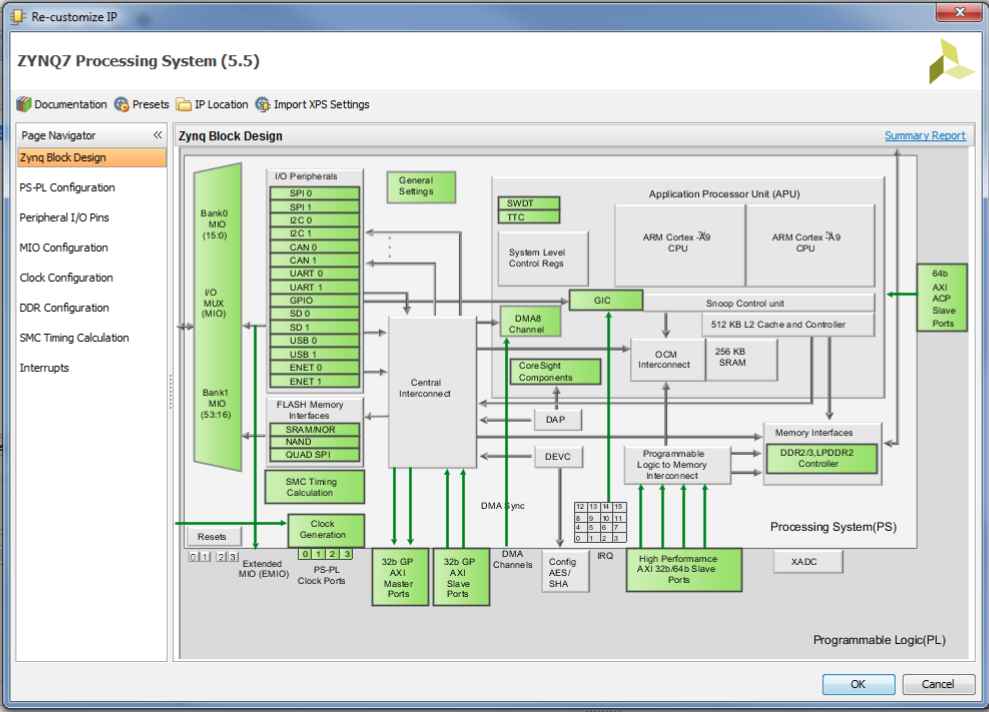
\includegraphics[width=1\textwidth]{zynq7ps.png}}
	\caption{Zynq7 Processing System Customization Window \cite{zynq7ps}}
	\label{zynq7ps_pic}
\end{figure}

There were two options for UART: UART0 and UART1. The functionality of UART0 and UART1 were nearly identical, except that UART1 had the capability of being routed to the ZedBoard's USB UART port, which was not compatible with the rangefinder \cite{zedboard_datasheet}. So, UART0 was arbitrarily chosen and the signals were routed to MIO10 and MIO11, which correspond to the ZedBoard's PS Pmod, JE.
\par
After choosing UART0 and configuring the MIO pins, the baud rate was configured to match the rangefinder's default communication speed of 19200 baud \cite{urg04lx_datasheet}. This was done in the processing system's customization window under PS-PL Configuration on the sidebar in Figure \ref{zynq7ps_pic}. Figure \ref{zynq7ps_baud_pic} shows the PS-PL Configuration window.

\begin{figure}[H]
	\centerline{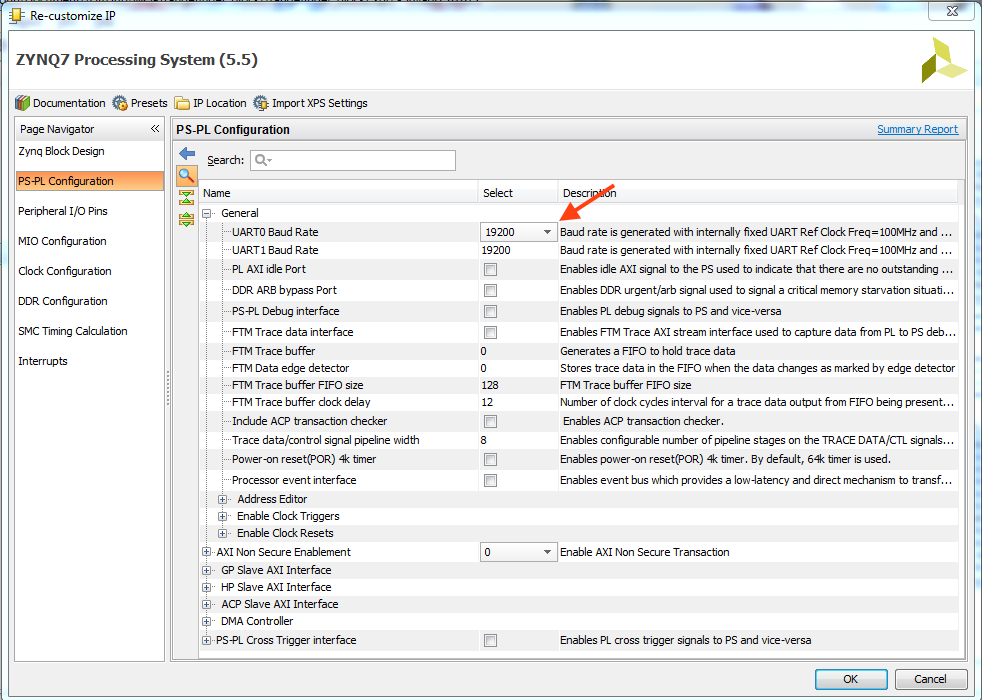
\includegraphics[width=1\textwidth]{zynq7ps_baud.png}}
	\caption{Zynq7 Processing System PS-PL Configuration Window}
	\label{zynq7ps_baud_pic}
\end{figure}

With the processing system customized in this fashion, the Programmable Logic's configuration for the rangefinder was complete.

\subsubsection{Designing with the Xilinx SDK}
The Programmable Software (PS) was coded in the Xilinx SDK. To launch the SDK, the hardware design was exported so that the PS had a platform to be coded on. This was done by generating a bitstream. The bitstream compiled all the project's hardware customization into a $.bit$ file which was used to program the FPGA on the ZedBoard. Generating a bitstream was done in Vivado under the Program and Debug section of the Flow Navigator, as seen in Figure \ref{generateBitstream}.

\begin{figure}[H]
	\centerline{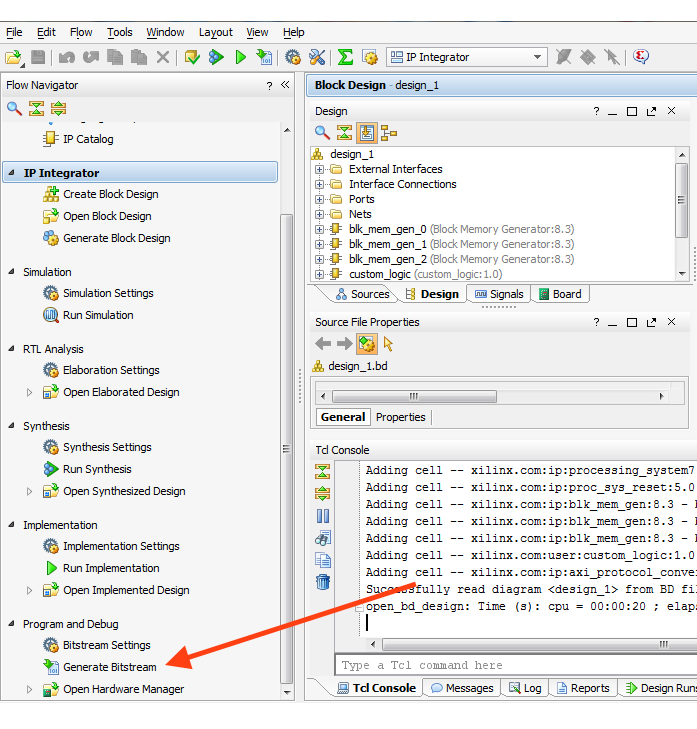
\includegraphics[width=.85\textwidth]{generateBitstream.png}}
	\caption{Generating a Bitstream in Vivado}
	\label{generateBitstream}
\end{figure}

Once the bitstream was generated, the design was exported to the SDK. This was done in Vivado by choosing File $\rightarrow$ Export $\rightarrow$ Export Hardware and including the bitstream. Finally, the SDK was launched by choosing File $\rightarrow$ Launch SDK.
\par
When the SDK launched, there was a hardware platform project in the Project Explorer tab. This file contained the hardware platform that was exported from Vivado and was used to program the FPGA on the ZedBoard. To begin programming the PS, an Application Project was created with the hardware platform by choosing File $\rightarrow$ New $\rightarrow$ Application Project, entering a project name, and choosing Next. Note that the hardware platform exported from Vivado was selected in the Hardware Platform and was used to create the Application Project. Next, a template was chosen to begin designing. For this project, the 'Hello World' template was chosen. This process is shown in Figure \ref{newApplicationProject}. The programmable software was edited in the project's source code file.

\begin{figure}[H]
	\centerline{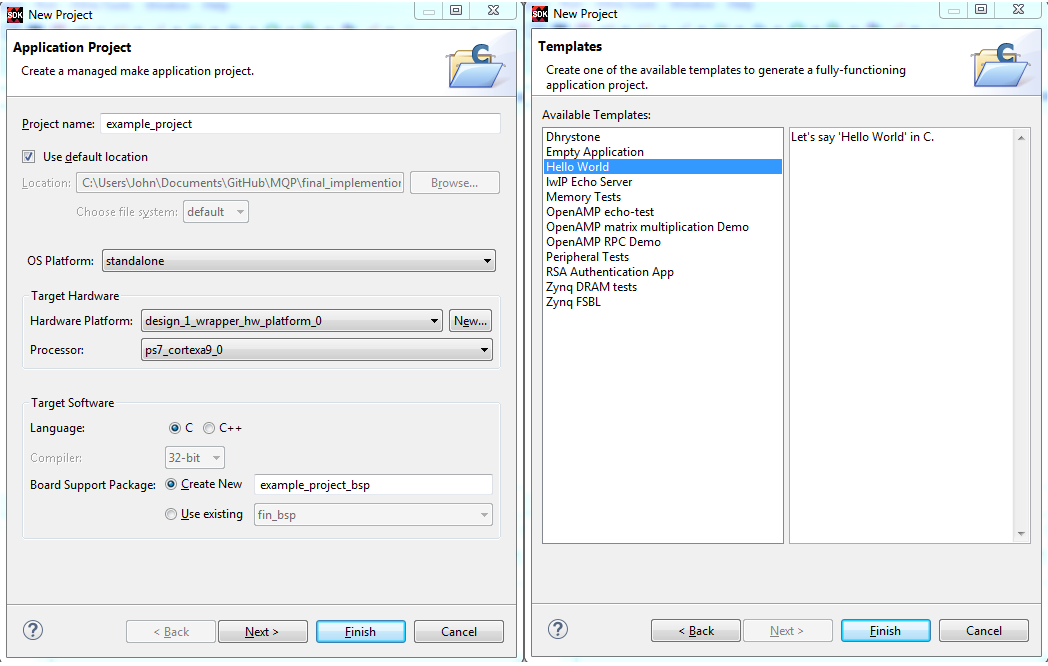
\includegraphics[width=1\textwidth]{newApplicationProject.png}}
	\caption{Creating a New Application Project in the Xilinx SDK}
	\label{newApplicationProject}
\end{figure}

To upload the design to the ZedBoard, the FPGA fabric of the SoC was programmed first in order to configure the PL with the hardware platform. This was done by choosing Xilinx Tools $\rightarrow$ Program FPGA. To indicate success, the ZedBoard's blue $DONE$ LED, LD12, illuminated. Once that process was completed, the PS was uploaded by right clicking on the application project then choosing Run As $\rightarrow$ Launch on Hardware (GDB).
\par
With an understanding of the rangefinder's interface, the data processing strategy was implemented. This will be explored in the following section.






